\documentclass{mylib/reporteConCalif}
\title{Reporte}
\author{rodrigofranciscopablo }

\subject{Laboratorio de Diseño Digital}
\mytitle{Reporte de práctica 4}
\mysubTitle{Circuito elevador de Bits al cuadrado}
\students{Francisco Pablo \textsc{Rodrigo}}
\teacher{M.I. Guevara Rodríguez \textsc{Ma. del Socorro}}
\group{6}
\deliverDate{11 de marzo de 2019}

\newcommand{\funx}{x_1(a,b,c,d) = [a \cdot \overline{b}(c+b \cdot d) + \overline{a} \cdot \overline{b} ]c}

\begin{document}

\coverPage

\tableofcontents
\newpage

\section{Objetivos}

\subsection{General}

El alumno diseñará circuitos combinacionales.

\subsection{Particular}

El alumno analizará, diseñará e implementará multifunciones algebraicas utilizando distintas formas
de optimización.

\section{Introducción}

Los circuitos combinacionales son, como su nombre lo sugiere, circuitos cuya salida depende solamente de la “combinación” de sus entradas en el momento que se está realizando la medición en la salida.
Los circuitos de lógica combinacional son hechos a partir de las compuertas básicas compuerta AND, compuerta OR, compuerta NOT. También pueden ser construidos con compuertas NAND, compuertas NOR, compuerta XOR, que son una combinación de las tres compuertas básicas.
La operación de los circuitos combinacionales se entienden escribiendo las ecuaciones booleanas y sus tablas de verdad.

Todos los circuitos combinacionales pueden representarse empleando álgebra de Boole a partir de su función lógica, generando de forma matemática el funcionamiento del sistema combinacional. De este modo, cada señal de entrada es una variable de la ecuación lógica de salida. \\

Por otra parte, la manipulación de funciones booleana puede llegar a ser muy compleja por lo cual se hace necesario el concepto de minimización. La minimización es básicamente la simplificación de una función, obteniendo una expresión que contenga menos términos o menos variables que la función original.  Esto se refleja en la obtención de circuito mas económicos por tener un menor numero de compuertas.



%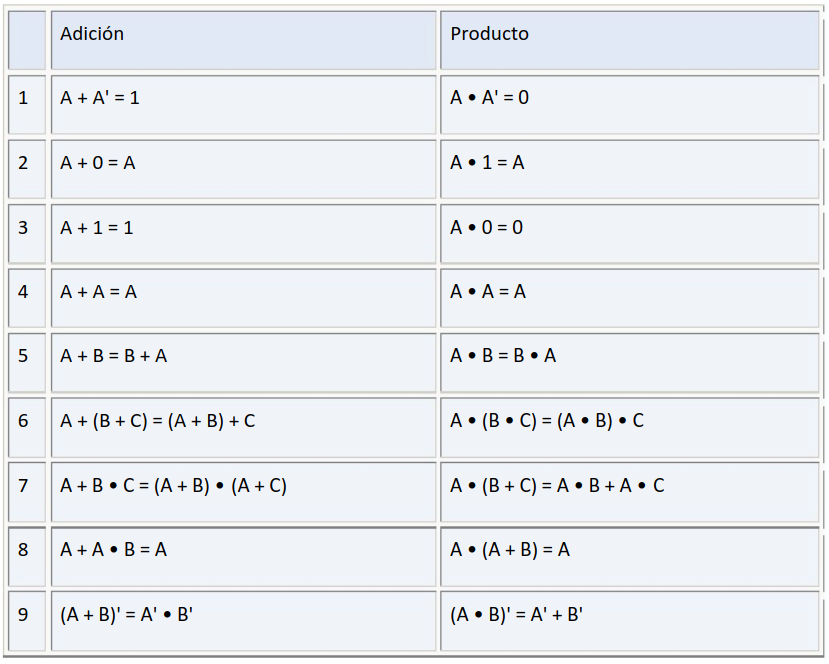
\includegraphics[width=8cm]{img/labdise_practica3/image9}

\newpage
\section{Previo}

\newpage
\section{Desarrollo}

Para el desarrollo de esta práctica construimos la funcion booleana $\funx$ en un diagrama esquemático de \textit{Xilinx} como se muestra acontinuación.\\

%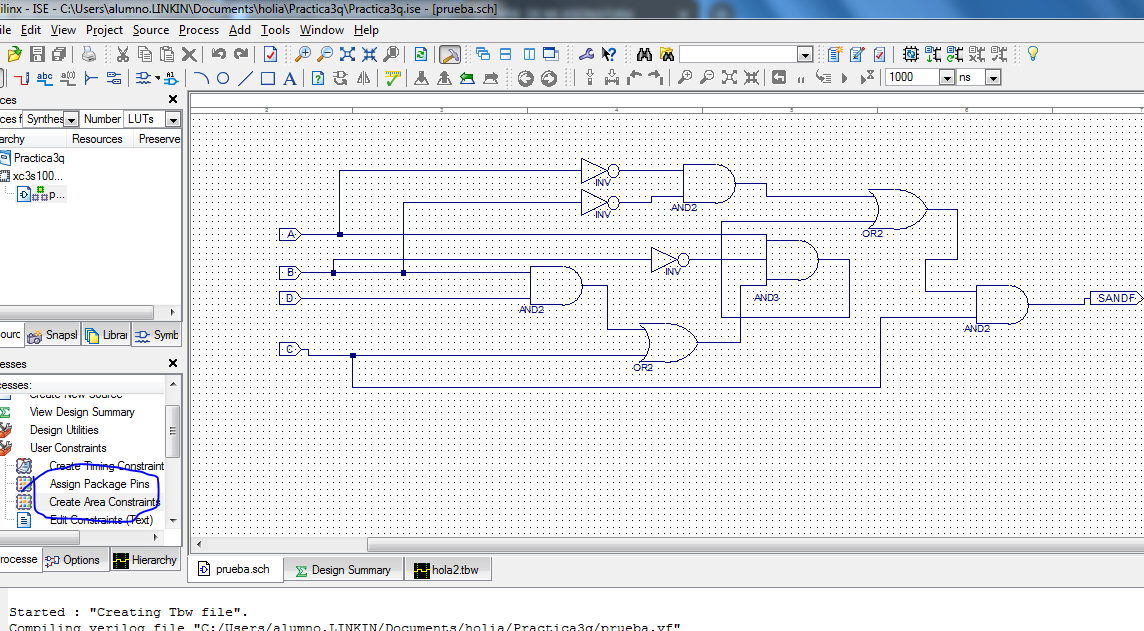
\includegraphics[width=15cm]{img/labdise_practica3/image10}\\

Luego debemos sintetizar nuestro programa para asegurarnos de que no haya errores y que las salidas sean efectivamente las que esperamos para lo cual recurrimos a la ventana que nos muestra un tren de pulsos como se observa a continuación.\\

%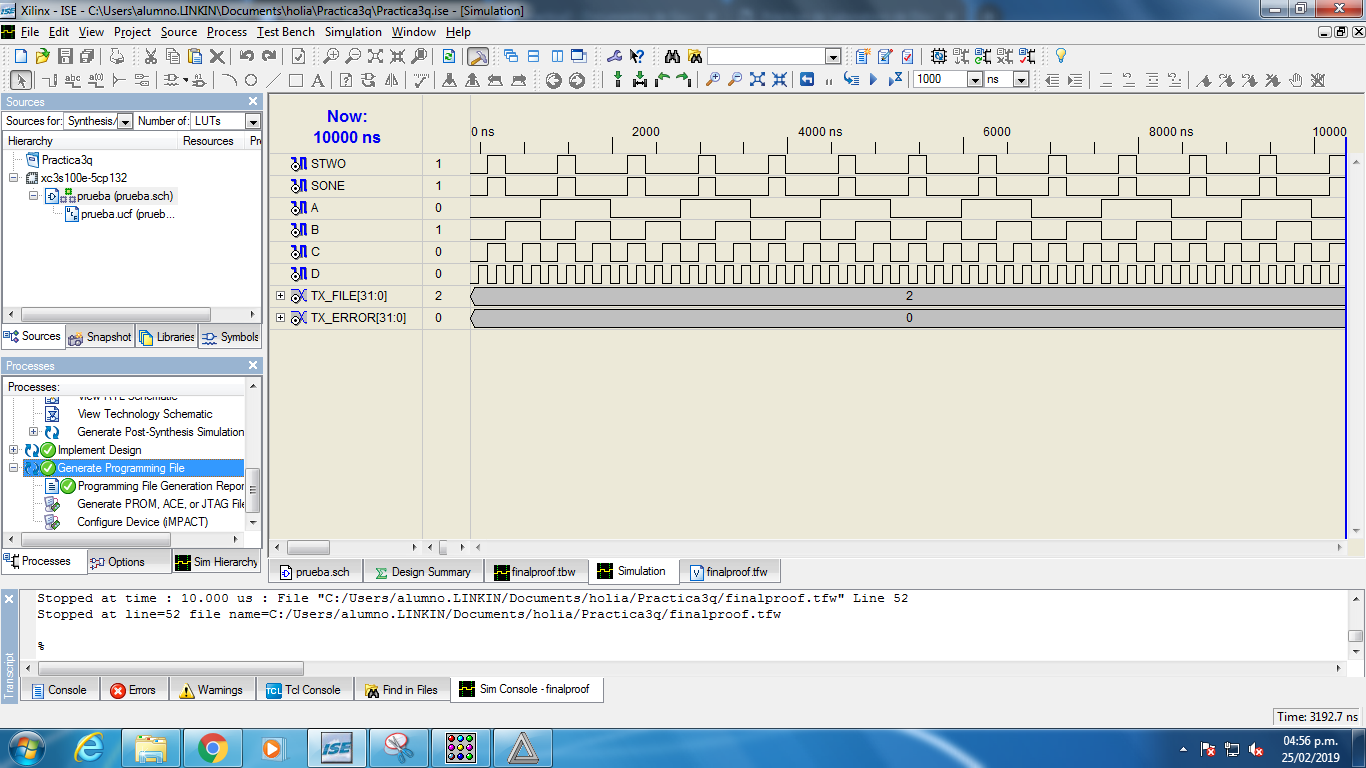
\includegraphics[width=15cm]{img/labdise_practica3/image4}\\

Una vez que nuestro diseño fue realizado correctamente procedemos a descargar el programa en la FPGA, para ello debemos indicarle al programa que queremos utilizar un \textit{Area Constraints} y en la ventana que se abrirá ligaremos los pines que vamos a usar del la FPGA con nuestro diseño.\\

%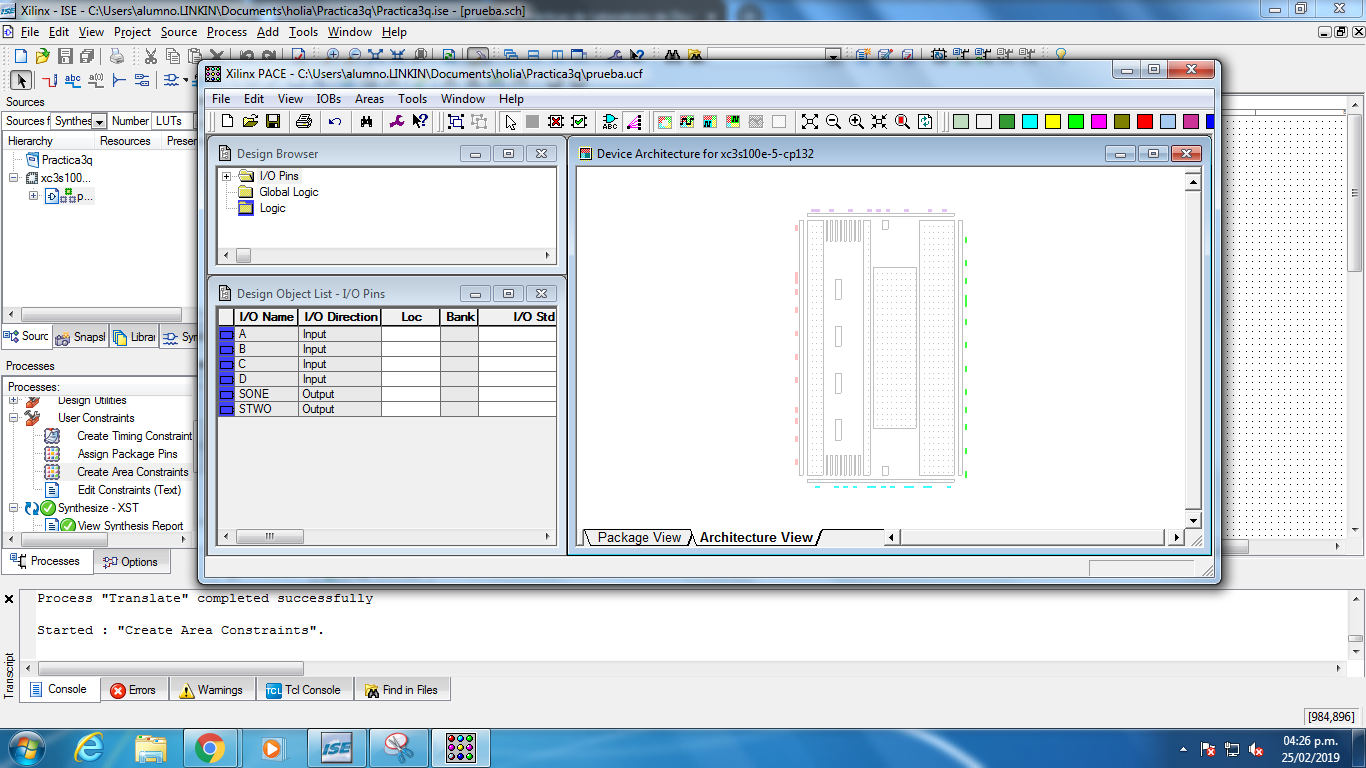
\includegraphics[width=15cm]{img/labdise_practica3/image7}\\

Finalmente para cargar el diseño a la FPGA, en nuestro caso utilizaremos la \textit{Basys o Spartan3E} para lo cual abriremos un programa llamado \textit{ADEPT} \\

%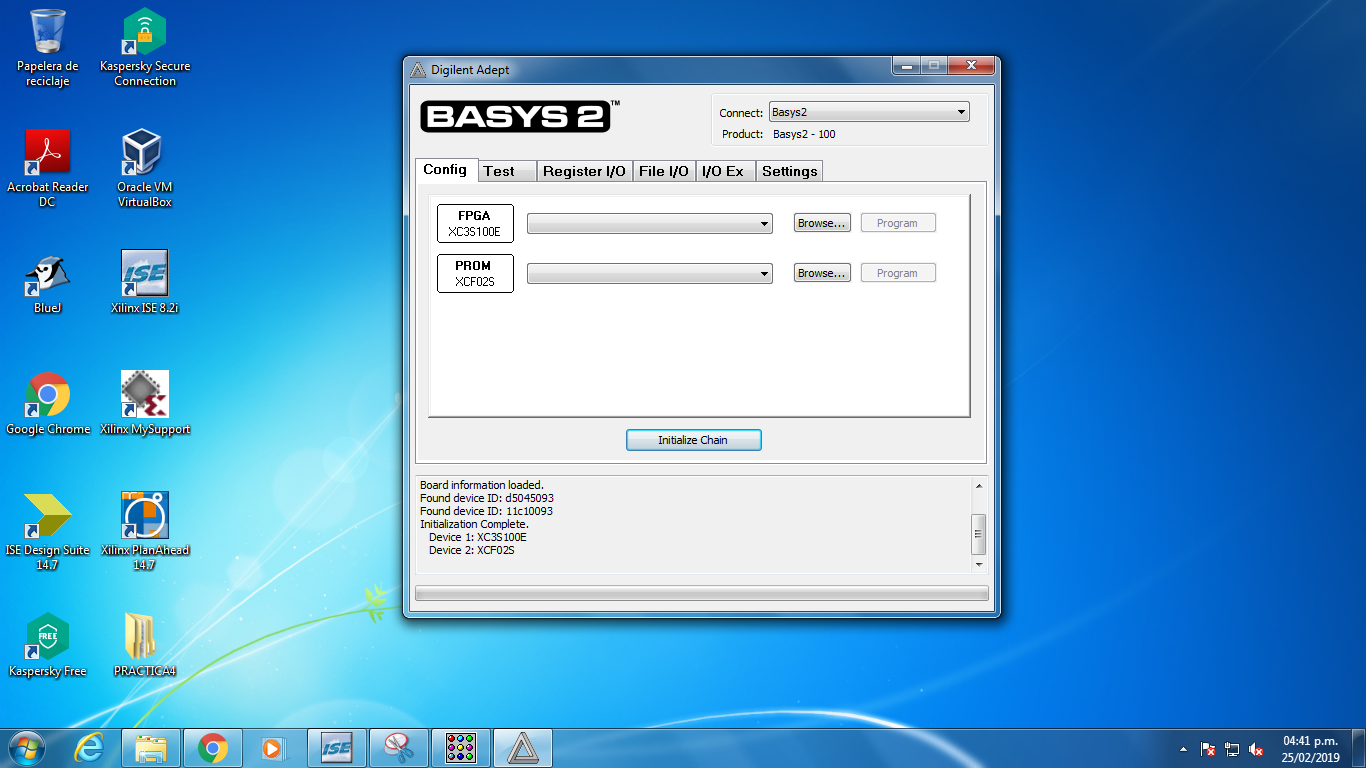
\includegraphics[width=15cm]{img/labdise_practica3/image5}\\

Conectamos la FPGA a nuestra computadora y verificamos que el programa la reconozca. \\

Finalmente debemos buscar el archivo que le cargaremos, dicho archivo fue producido por nuestro programa Xilinx y tiene extensión .bit. Una vez que lo encontremos los seleccionamos y cargamos dicho programa a la tarjeta.\\

%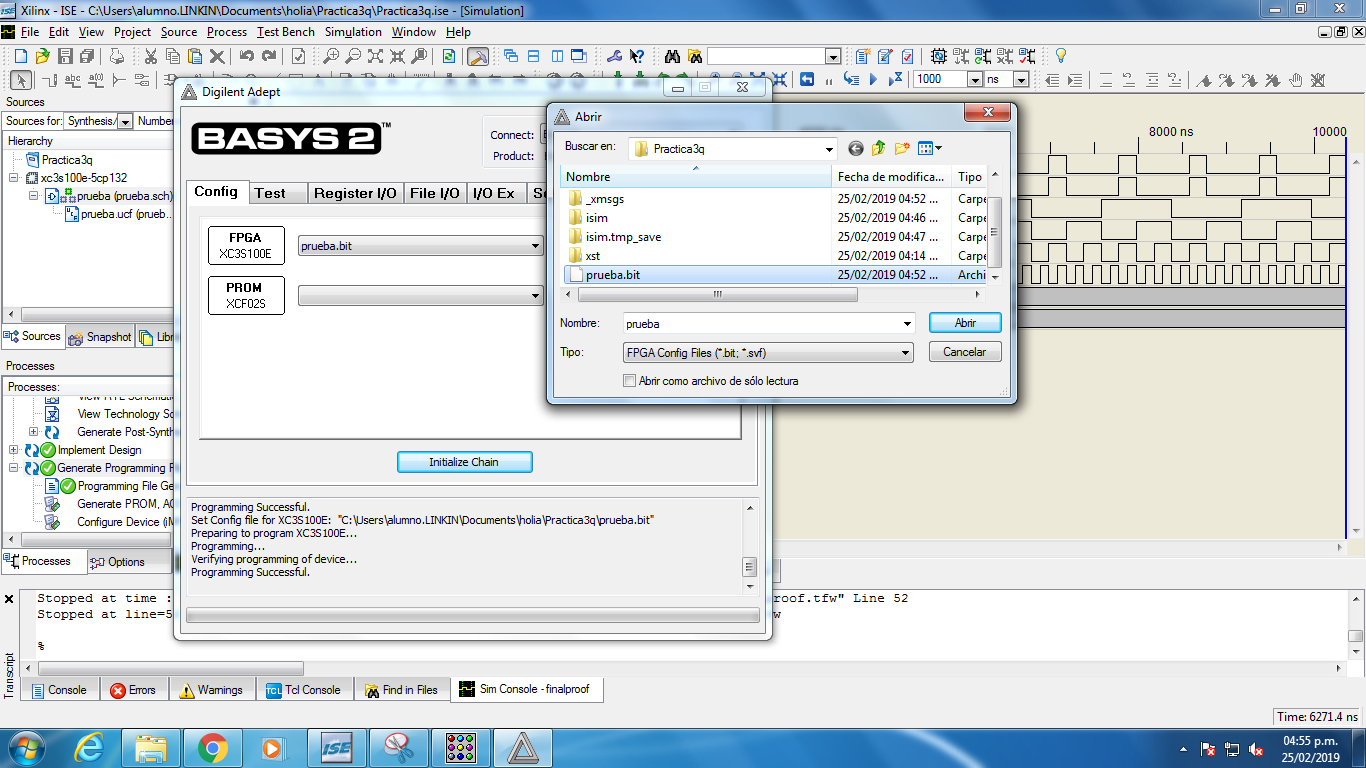
\includegraphics[width=15cm]{img/labdise_practica3/image1}\\

Ahora tenemos nuestro primer programa cargado en la FPGA y puede verse como tiene dos LEDS encendidos que también podrían estar apagados de acuerdo a la configuración de los switches de abajo.\\

%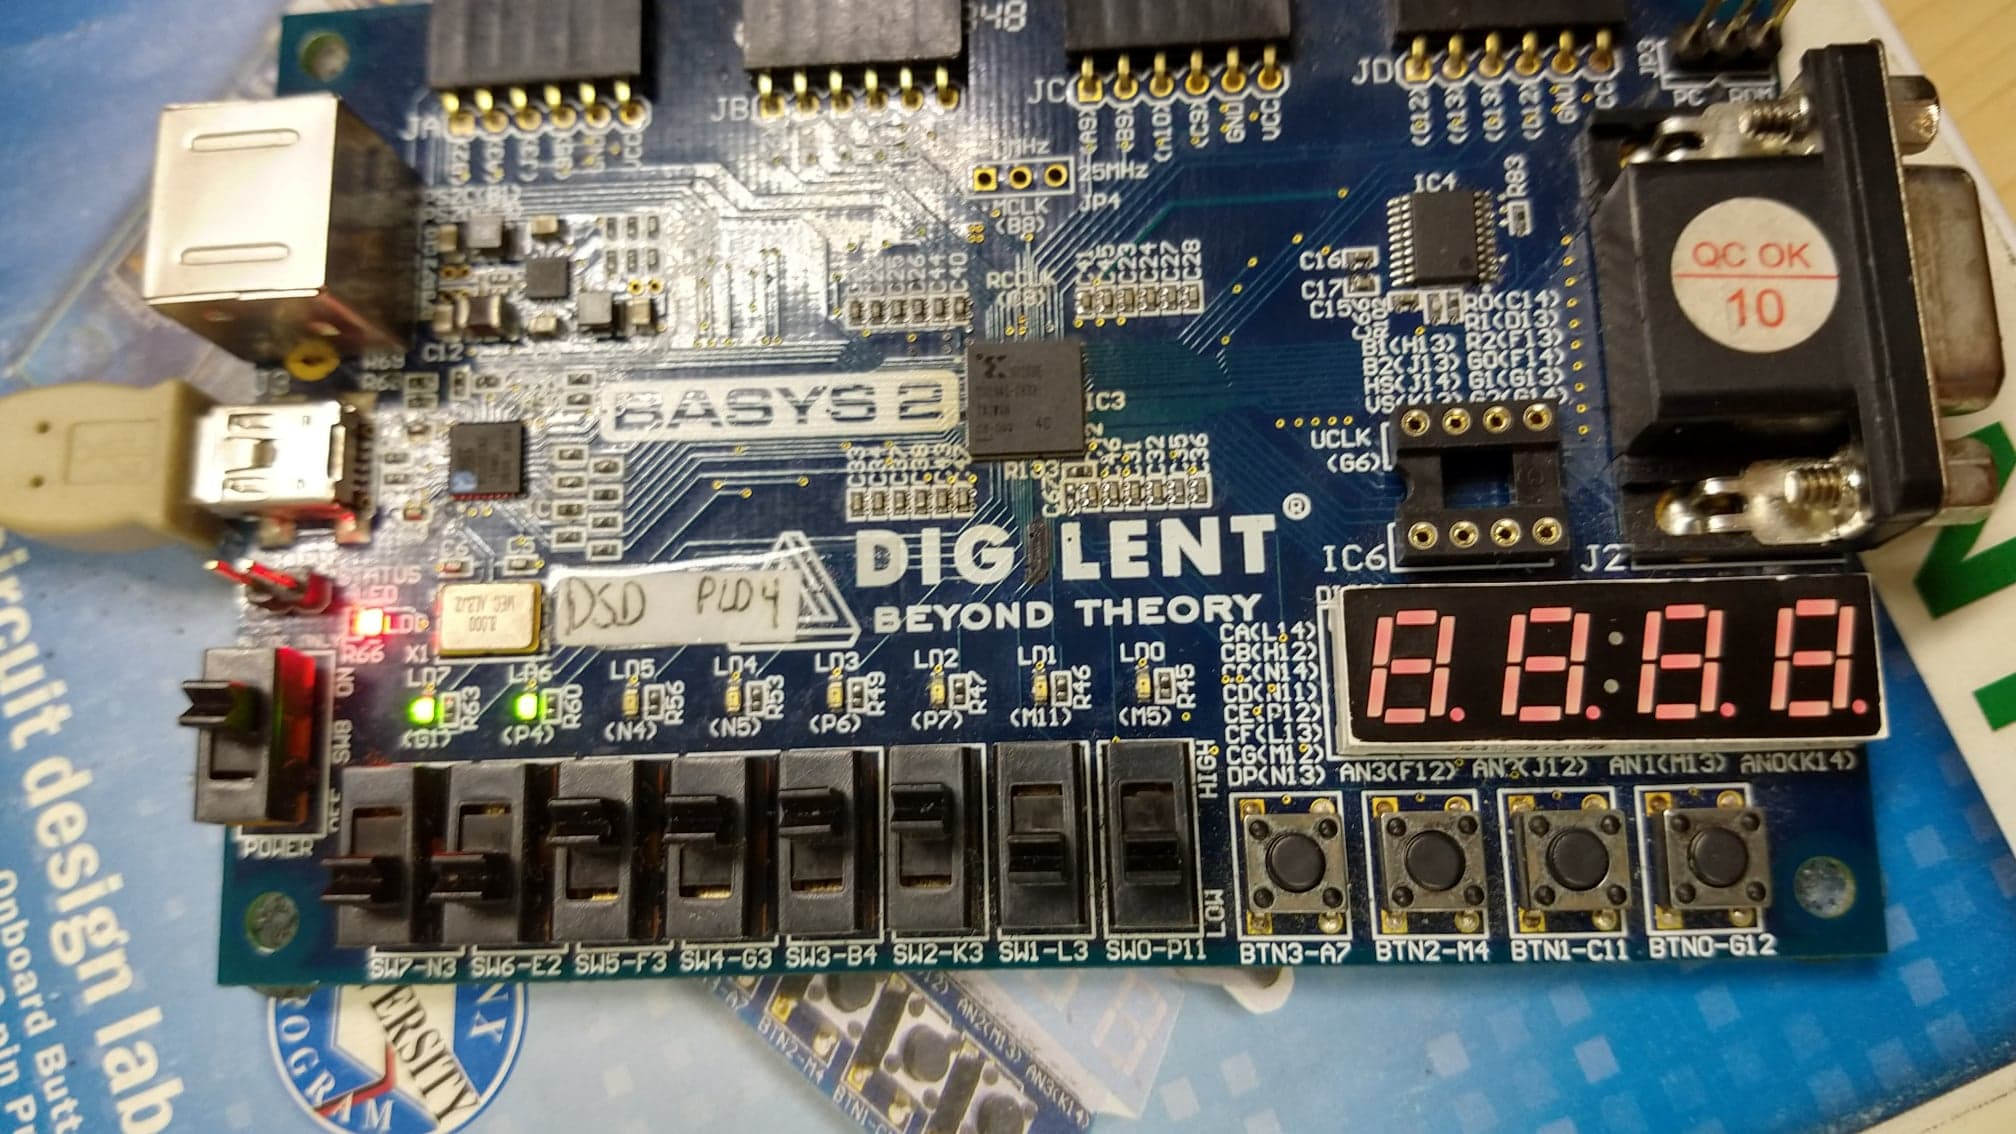
\includegraphics[width=15cm]{img/labdise_practica3/funciona}\\

\section{Conclusiones}

Tener una FPGA hace que solo nos preocupemos por el desarrollo de nuestro circuito ya que si no la tuvieramos tendríamos que tener algunos circuitos integrados (compuertas AND y OR), alambre, botones, LEDs y alguna que otra resistencia. Además de que el tiempo de armado sería como alrededor de dos o tres horas, en cambio con la tajeta que ya tiene todo integrado nos tardadamos como media hora y eso considerando que somos usuarios que apenas estan aprendiendo a usarla.\\

Finalmente esta práctica ayudo a entender de manera más puntual como es que funciona el Algebra de Boole y su relación con la electrónica. Al inicio de la práctica ya sabíamos hacer álgebra de Boole sin embargo no entendiamos del todo bien como aplicarla, después de la práctica nos damos cuenta de su importancia en el mundo electrónico.

\end{document}